\documentclass[11pt,a4paper]{article}

\usepackage[margin=2.2cm]{geometry}
\usepackage{graphicx}
\usepackage{float}
\usepackage{booktabs}
\usepackage{xcolor}
\usepackage{hyperref}
\usepackage{tikz}
\usetikzlibrary{shapes.geometric, arrows.meta, positioning, fit, calc}
\usepackage{enumitem}
\usepackage{fancyhdr}
\usepackage{titlesec}
\usepackage{caption}
\usepackage{subcaption}
\usepackage{amsmath}
\usepackage{amssymb}

\hypersetup{colorlinks=true, linkcolor=blue!60!black, urlcolor=blue!60!black}

\definecolor{completed}{HTML}{2E8B57}
\definecolor{inprogress}{HTML}{D4822F}
\definecolor{stagebox}{HTML}{E8EEF4}
\definecolor{resultbox}{HTML}{FFF8E1}

\pagestyle{fancy}
\fancyhf{}
\rhead{\small Progress Report --- August 2026}
\lhead{\small Ali Azizpourian}
\cfoot{\thepage}

\titleformat{\section}{\large\bfseries}{\thesection}{1em}{}
\titleformat{\subsection}{\normalsize\bfseries}{\thesubsection}{1em}{}

\title{\textbf{Master's Thesis --- Progress Report}\\[6pt]
\large Key-Value Pair Extraction from Business Documents:\\
A Discriminative Layout-Aware Approach on KVP10k}
\author{Ali Azizpourian\\[2pt]
\small Friedrich-Alexander-Universit\"at Erlangen-N\"urnberg}
\date{18 August 2026}

\begin{document}
\maketitle
\thispagestyle{fancy}

% ============================================================
\section{Thesis Recap}
% ============================================================

This thesis investigates \textbf{key-value pair (KVP) extraction} from semi-structured documents (invoices, receipts, forms) using IBM's \textbf{KVP10k} benchmark dataset (ICDAR 2024, Naparstek et al.).
The KVP10k paper argued that encoder-based models such as LayoutLMv3 have limitations for direct KVP linking, and therefore evaluated only a generative LMDX-style baseline rather than empirically benchmarking LayoutLMv3 on KVP10k.

This thesis evaluates a generative baseline and an adaptation of a pretrained
LayoutLMv3 encoder with an explicit relation linker. The final research questions are:

\begin{enumerate}[nosep]
  \item \textbf{RQ1:} How do layout characteristics vary across business documents, and how can this inform model design?
  \item \textbf{RQ2:} How does a LayoutLMv3-based discriminative linker perform on regular KVP extraction compared with a generative baseline?
  \item \textbf{RQ3:} What does the experimental progression from token-level to span-level linking reveal about key--value association?
  \item \textbf{RQ4:} Which factors characterise model successes and failures across page-level annotation-geometry regimes?
\end{enumerate}

The project is organized into five stages (Figure~\ref{fig:pipeline}).
All five stages, including final V5 training and evaluation, are complete.

\begin{figure}[ht]
\centering
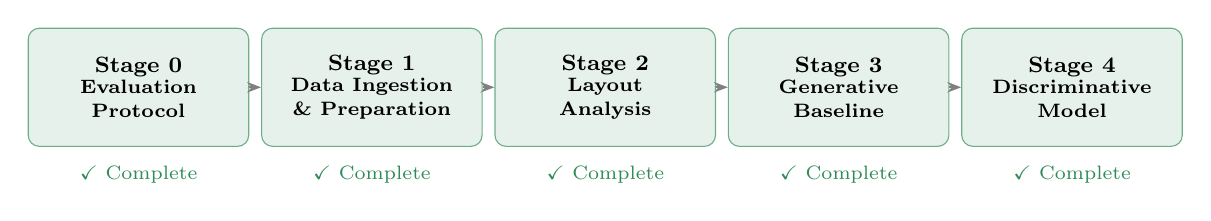
\begin{tikzpicture}[
  node distance=0.15cm and 0.15cm,
  stage/.style={
    rectangle, rounded corners=4pt, draw=black!60,
    fill=stagebox, minimum width=2.8cm, minimum height=1.5cm,
    align=center, font=\footnotesize\bfseries
  },
  done/.style={stage, draw=completed!70, fill=completed!12},
  arr/.style={-{Stealth[length=5pt]}, thick, black!50}
]
  \node[done] (s0) {Stage 0\\[-2pt]\scriptsize Evaluation\\[-1pt]\scriptsize Protocol};
  \node[done, right=of s0] (s1) {Stage 1\\[-2pt]\scriptsize Data Ingestion\\[-1pt]\scriptsize \& Preparation};
  \node[done, right=of s1] (s2) {Stage 2\\[-2pt]\scriptsize Layout\\[-1pt]\scriptsize Analysis};
  \node[done, right=of s2] (s3) {Stage 3\\[-2pt]\scriptsize Generative\\[-1pt]\scriptsize Baseline};
  \node[done, right=of s3]  (s4) {Stage 4\\[-2pt]\scriptsize Discriminative\\[-1pt]\scriptsize Model};

  \draw[arr] (s0) -- (s1);
  \draw[arr] (s1) -- (s2);
  \draw[arr] (s2) -- (s3);
  \draw[arr] (s3) -- (s4);

  \node[below=0.12cm of s0, font=\scriptsize\color{completed}] {\checkmark\ Complete};
  \node[below=0.12cm of s1, font=\scriptsize\color{completed}] {\checkmark\ Complete};
  \node[below=0.12cm of s2, font=\scriptsize\color{completed}] {\checkmark\ Complete};
  \node[below=0.12cm of s3, font=\scriptsize\color{completed}] {\checkmark\ Complete};
  \node[below=0.12cm of s4, font=\scriptsize\color{completed}] {\checkmark\ Complete};
\end{tikzpicture}
\caption{Pipeline overview. All five stages are complete.}
\label{fig:pipeline}
\end{figure}

% ============================================================
\section{Completed Work (Stages 0--4)}
% ============================================================

\subsection{Stage 0: Evaluation Protocol}
The evaluation protocol is adopted directly from the KVP10k paper (Naparstek et al., ICDAR 2024):
\begin{itemize}[nosep]
  \item \textbf{Text-only:} Normalized Edit Distance (NED) $< 0.2$ between predicted and ground-truth text.
  \item \textbf{Text + Location:} NED $< 0.2$ \emph{and} bounding-box IoU $\ge 0.3$.
\end{itemize}

\noindent The primary metric is \textbf{F1} (harmonic mean of precision and recall), and all linking results are reported under both metrics above. A key-value pair counts as correct only if \emph{both} its key and its value satisfy the criterion. The score uses the same metric definition as the published baseline, but the numerical comparison is contextual because the available pages and preprocessing pipelines differ.

\noindent
The IoU threshold of $0.3$ is adopted directly from Naparstek et al.\ (2024), who chose this value to permit minor spatial imprecision in predicted bounding boxes while still ensuring that the prediction is located in the correct spatial region of the page.
The paper describes an exceedance criterion, whereas the released IBM evaluator implements the boundary inclusively ($\mathrm{IoU}\ge 0.3$). This report follows the released implementation consistently.

\subsection{Stage 1: Data Ingestion \& Preparation}

The raw KVP10k dataset required substantial preparation before model training:

\begin{enumerate}[nosep, leftmargin=1.5em]
  \item \textbf{Deduplication:} Pages grouped by \texttt{hash\_name}; richest annotation selected. Raw 48{,}280 train rows $\to$ 9{,}656 unique pages; 5{,}255 test rows $\to$ 1{,}051 unique pages.
  \item \textbf{PDF download \& validation:} Source PDFs downloaded and verified per unique page.
  \item \textbf{Text extraction:} PyMuPDF used to extract words and bounding boxes. Pages without text layers discarded.
  \item \textbf{Annotation fusion:} Words matched against annotation bounding boxes to assign Key/Value/Other labels and reconstruct KVP link supervision.
  \item \textbf{LMDX formatting:} Each word encoded as \texttt{word x1|y1|x2|y2} in normalised coordinates.
\end{enumerate}

\begin{center}
\begin{tabular}{lcccl}
\toprule
\textbf{Split} & \textbf{Raw Rows} & \textbf{Unique Pages} & \textbf{Prepared Pages} & \textbf{Coverage} \\
\midrule
Train & 48{,}280 & 9{,}656 & 5{,}389 & 55.8\% \\
Test  & 5{,}255  & 1{,}051 & 581    & 55.3\% \\
\bottomrule
\end{tabular}
\end{center}

\noindent\textbf{Ground truth.} The key/value labels are \emph{not} produced by us: KVP10k ships human annotations (each key and value region, its text, and the key$\to$value link). Our preparation only \emph{reconstructs the word-level supervision} by fusing those annotations with PyMuPDF-extracted words.

\noindent\textbf{Data loss ($\sim$45\%).} The pages not prepared are lost overwhelmingly to \emph{broken or inaccessible source-PDF links} (the dataset ships URLs, not the PDFs themselves), not to filtering. Only a small minority are scanned pages with no digital text layer --- these are the only losses attributable to using PyMuPDF text extraction instead of Tesseract OCR. The preparation code does not separate the two causes, so an exact split is not recorded.

\subsection{Stage 2: Layout Clustering \& Analysis}

The final Stage~2 analysis operates on unique pages, not duplicated annotator
rows. Training rows were grouped by page hash and the annotation copy with the
most usable polygon coordinates was retained. Of 9{,}656 unique training pages,
9{,}124 contain usable geometry; the remaining 532 are excluded rather than
encoded as zero vectors. The historical \texttt{density} feature was removed
because it exactly duplicated \texttt{total\_area}, leaving 12 distinct
features standardized with \texttt{StandardScaler}.

K-means used seed 42 and 10 initializations. A sweep over
$k=2,\ldots,10$ selected $k=2$ by the predefined silhouette criterion
($0.222$); Calinski--Harabasz also favored $k=2$, while Davies--Bouldin
continued improving at larger $k$. Thus, the groups are exploratory geometry
strata rather than sharply separated semantic document classes.

\begin{figure}[H]
    \centering
    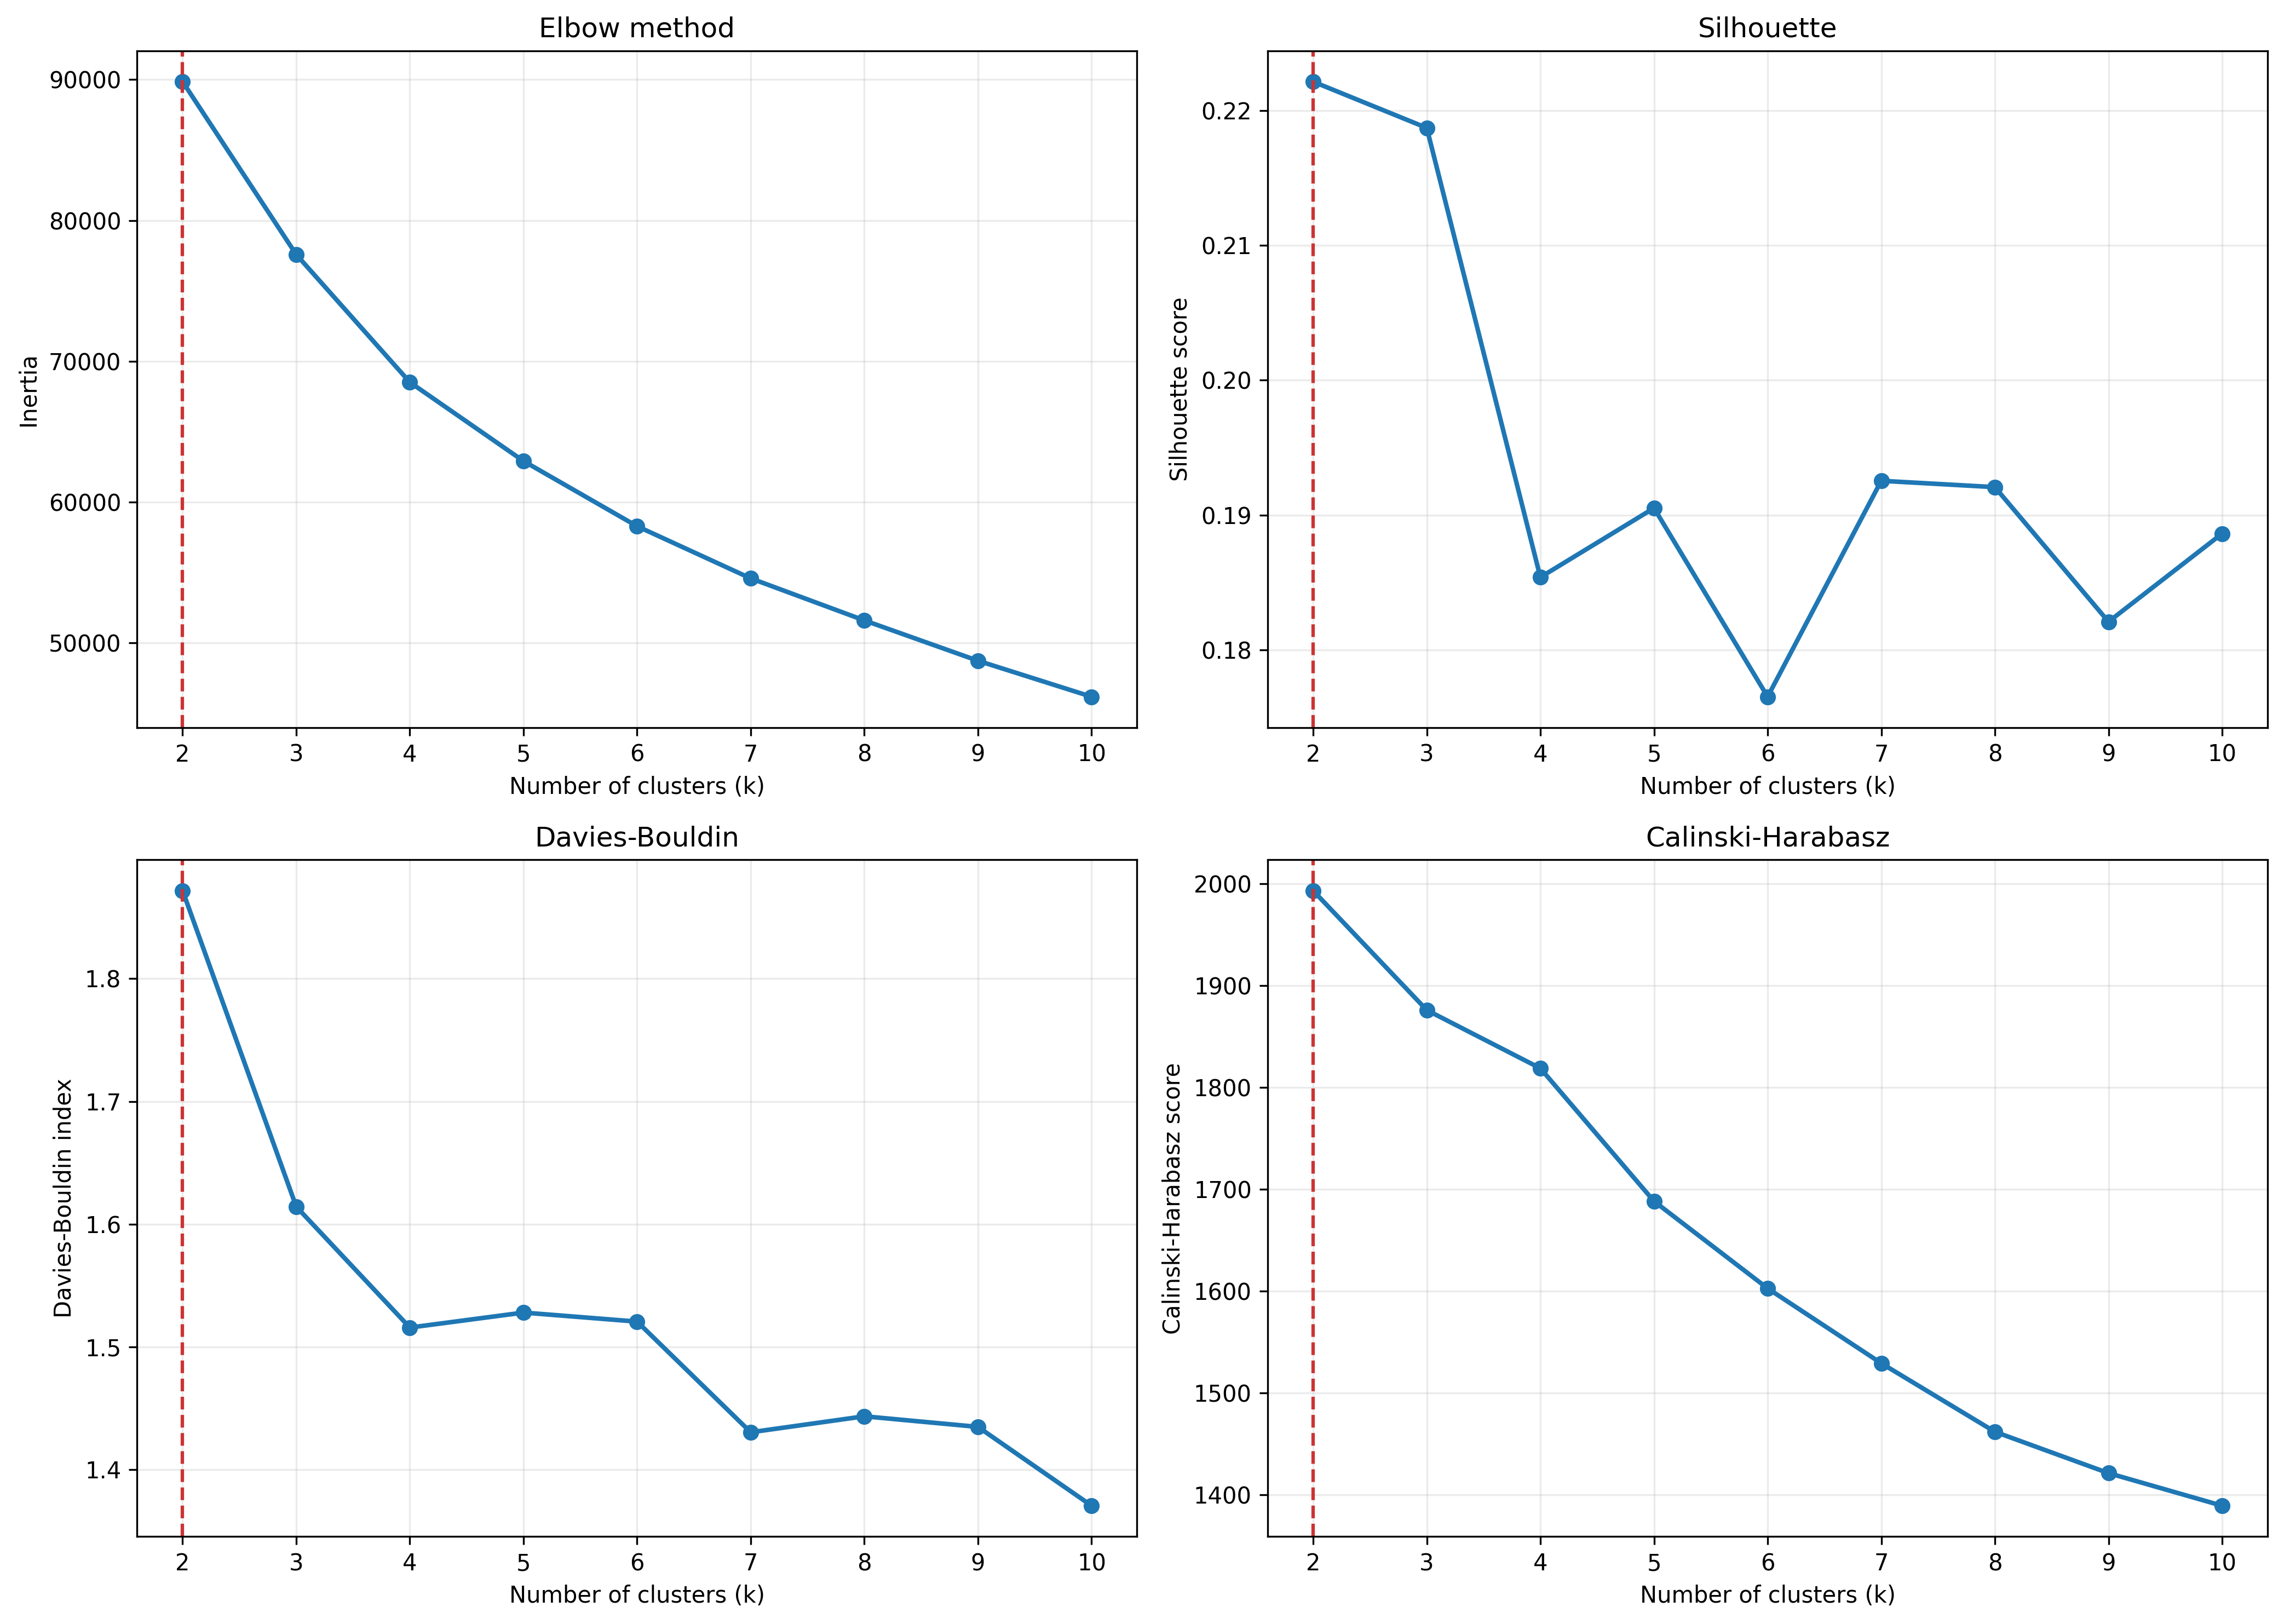
\includegraphics[width=0.72\textwidth]{figures/optimal_k_analysis.png}
    \caption{Final Stage~2 cluster-number analysis. The silhouette score is the
    primary selection criterion; the other diagnostics show that separation is
    modest and should not be over-interpreted.}
    \label{fig:pr-optimal-k}
\end{figure}

\begin{center}
\begin{tabular}{lccl}
\toprule
\textbf{Cluster} & \textbf{Pages} & \textbf{Share} & \textbf{Geometric character} \\
\midrule
0 & 5{,}617 & 61.6\% & Higher box count, broad spread \\
1 & 3{,}507 & 38.4\% & Lower box count, larger boxes, compact spread \\
\bottomrule
\end{tabular}
\end{center}

\begin{figure}[H]
    \centering
    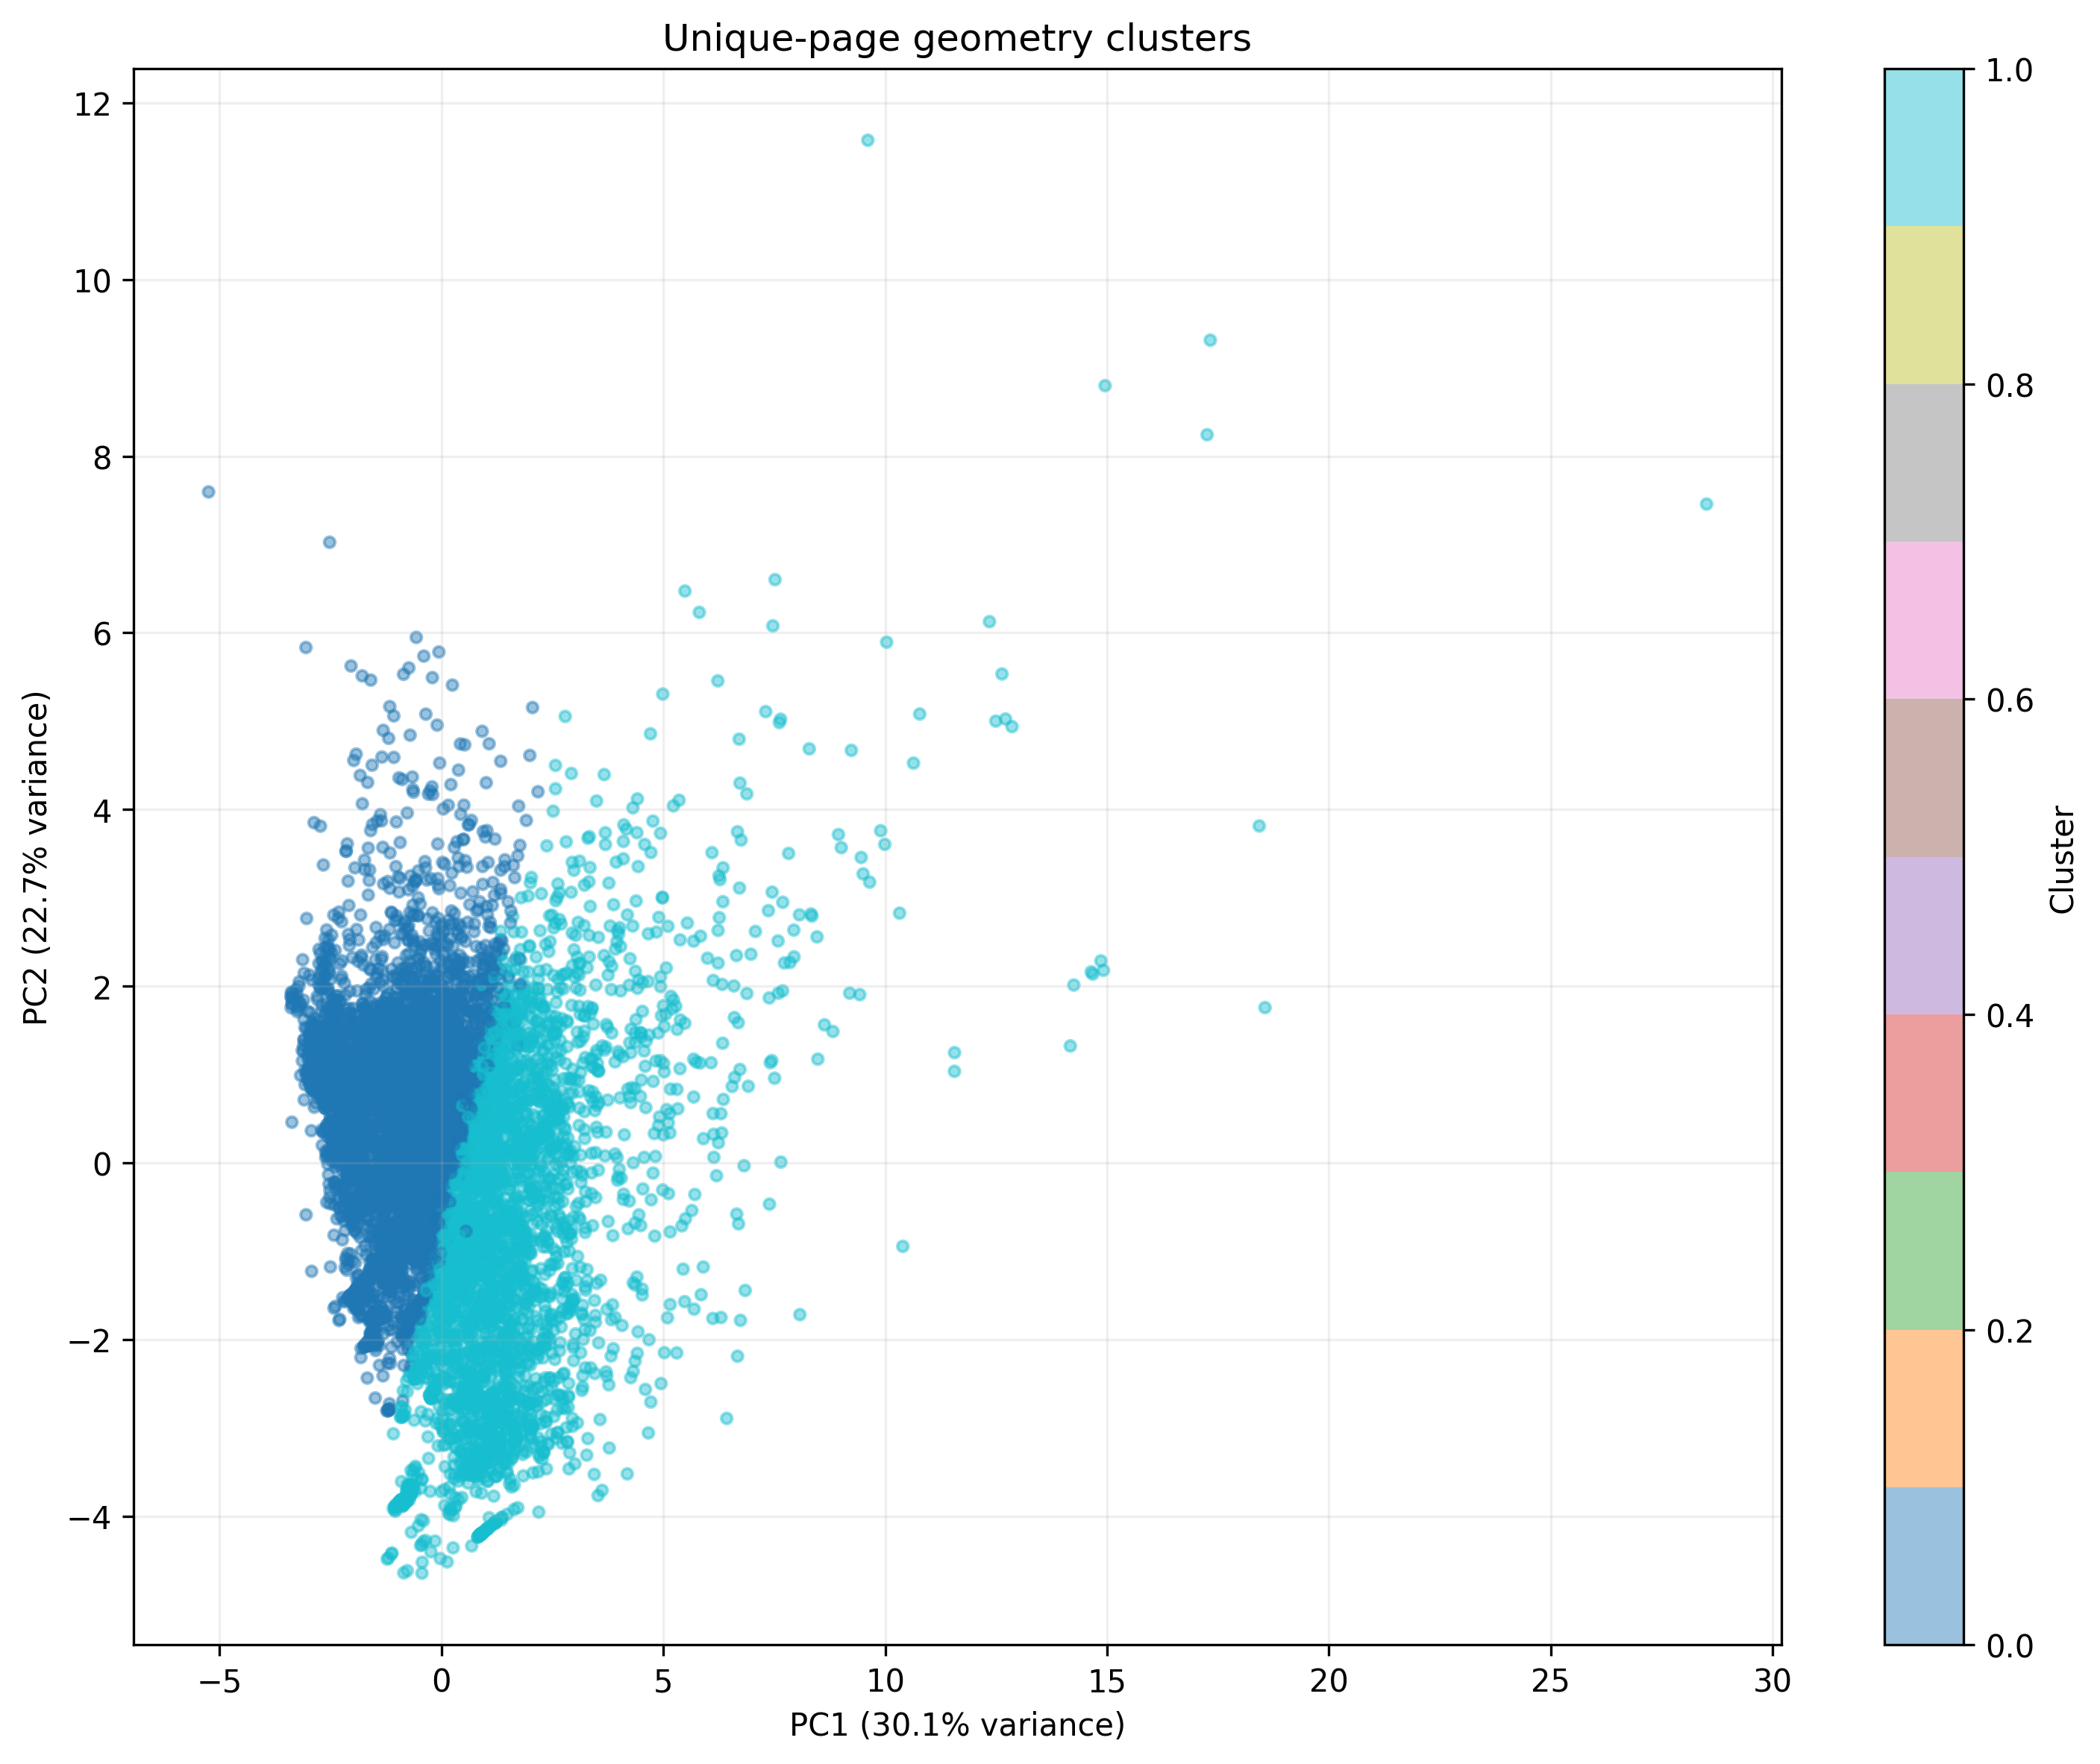
\includegraphics[width=0.72\textwidth]{figures/pca_clusters.png}
    \caption{Final PCA projection of the $k=2$ unique-page geometry clusters.
    PC1 and PC2 explain 30.15\% and 22.68\% of standardized-feature variance
    (52.83\% together). The visible overlap is consistent with the modest
    silhouette score.}
    \label{fig:pr-clusters-pca}
\end{figure}

\begin{figure}[H]
    \centering
    
\includegraphics[width=0.88\textwidth]{figures/stage2_cluster_examples.png}
    \caption{Representative test pages with annotation polygons. Cluster~0 is
    the higher-count, broader-spread regime; Cluster~1 is lower-count and more
    compact. These are geometry examples, not document-genre labels.}
    \label{fig:pr-cluster-examples}
\end{figure}

\noindent\textbf{Interpretation.} Cluster~0 averages
$31.659\pm22.460$ boxes with vertical/horizontal spread
$0.714\pm0.261$/$0.739\pm0.122$; Cluster~1 averages
$14.206\pm10.016$ boxes and spread
$0.421\pm0.289$/$0.372\pm0.202$. These statistics concern annotation-box
geometry, not OCR-token density, document genre, or general visual appearance.

\begin{figure}[H]
    \centering
    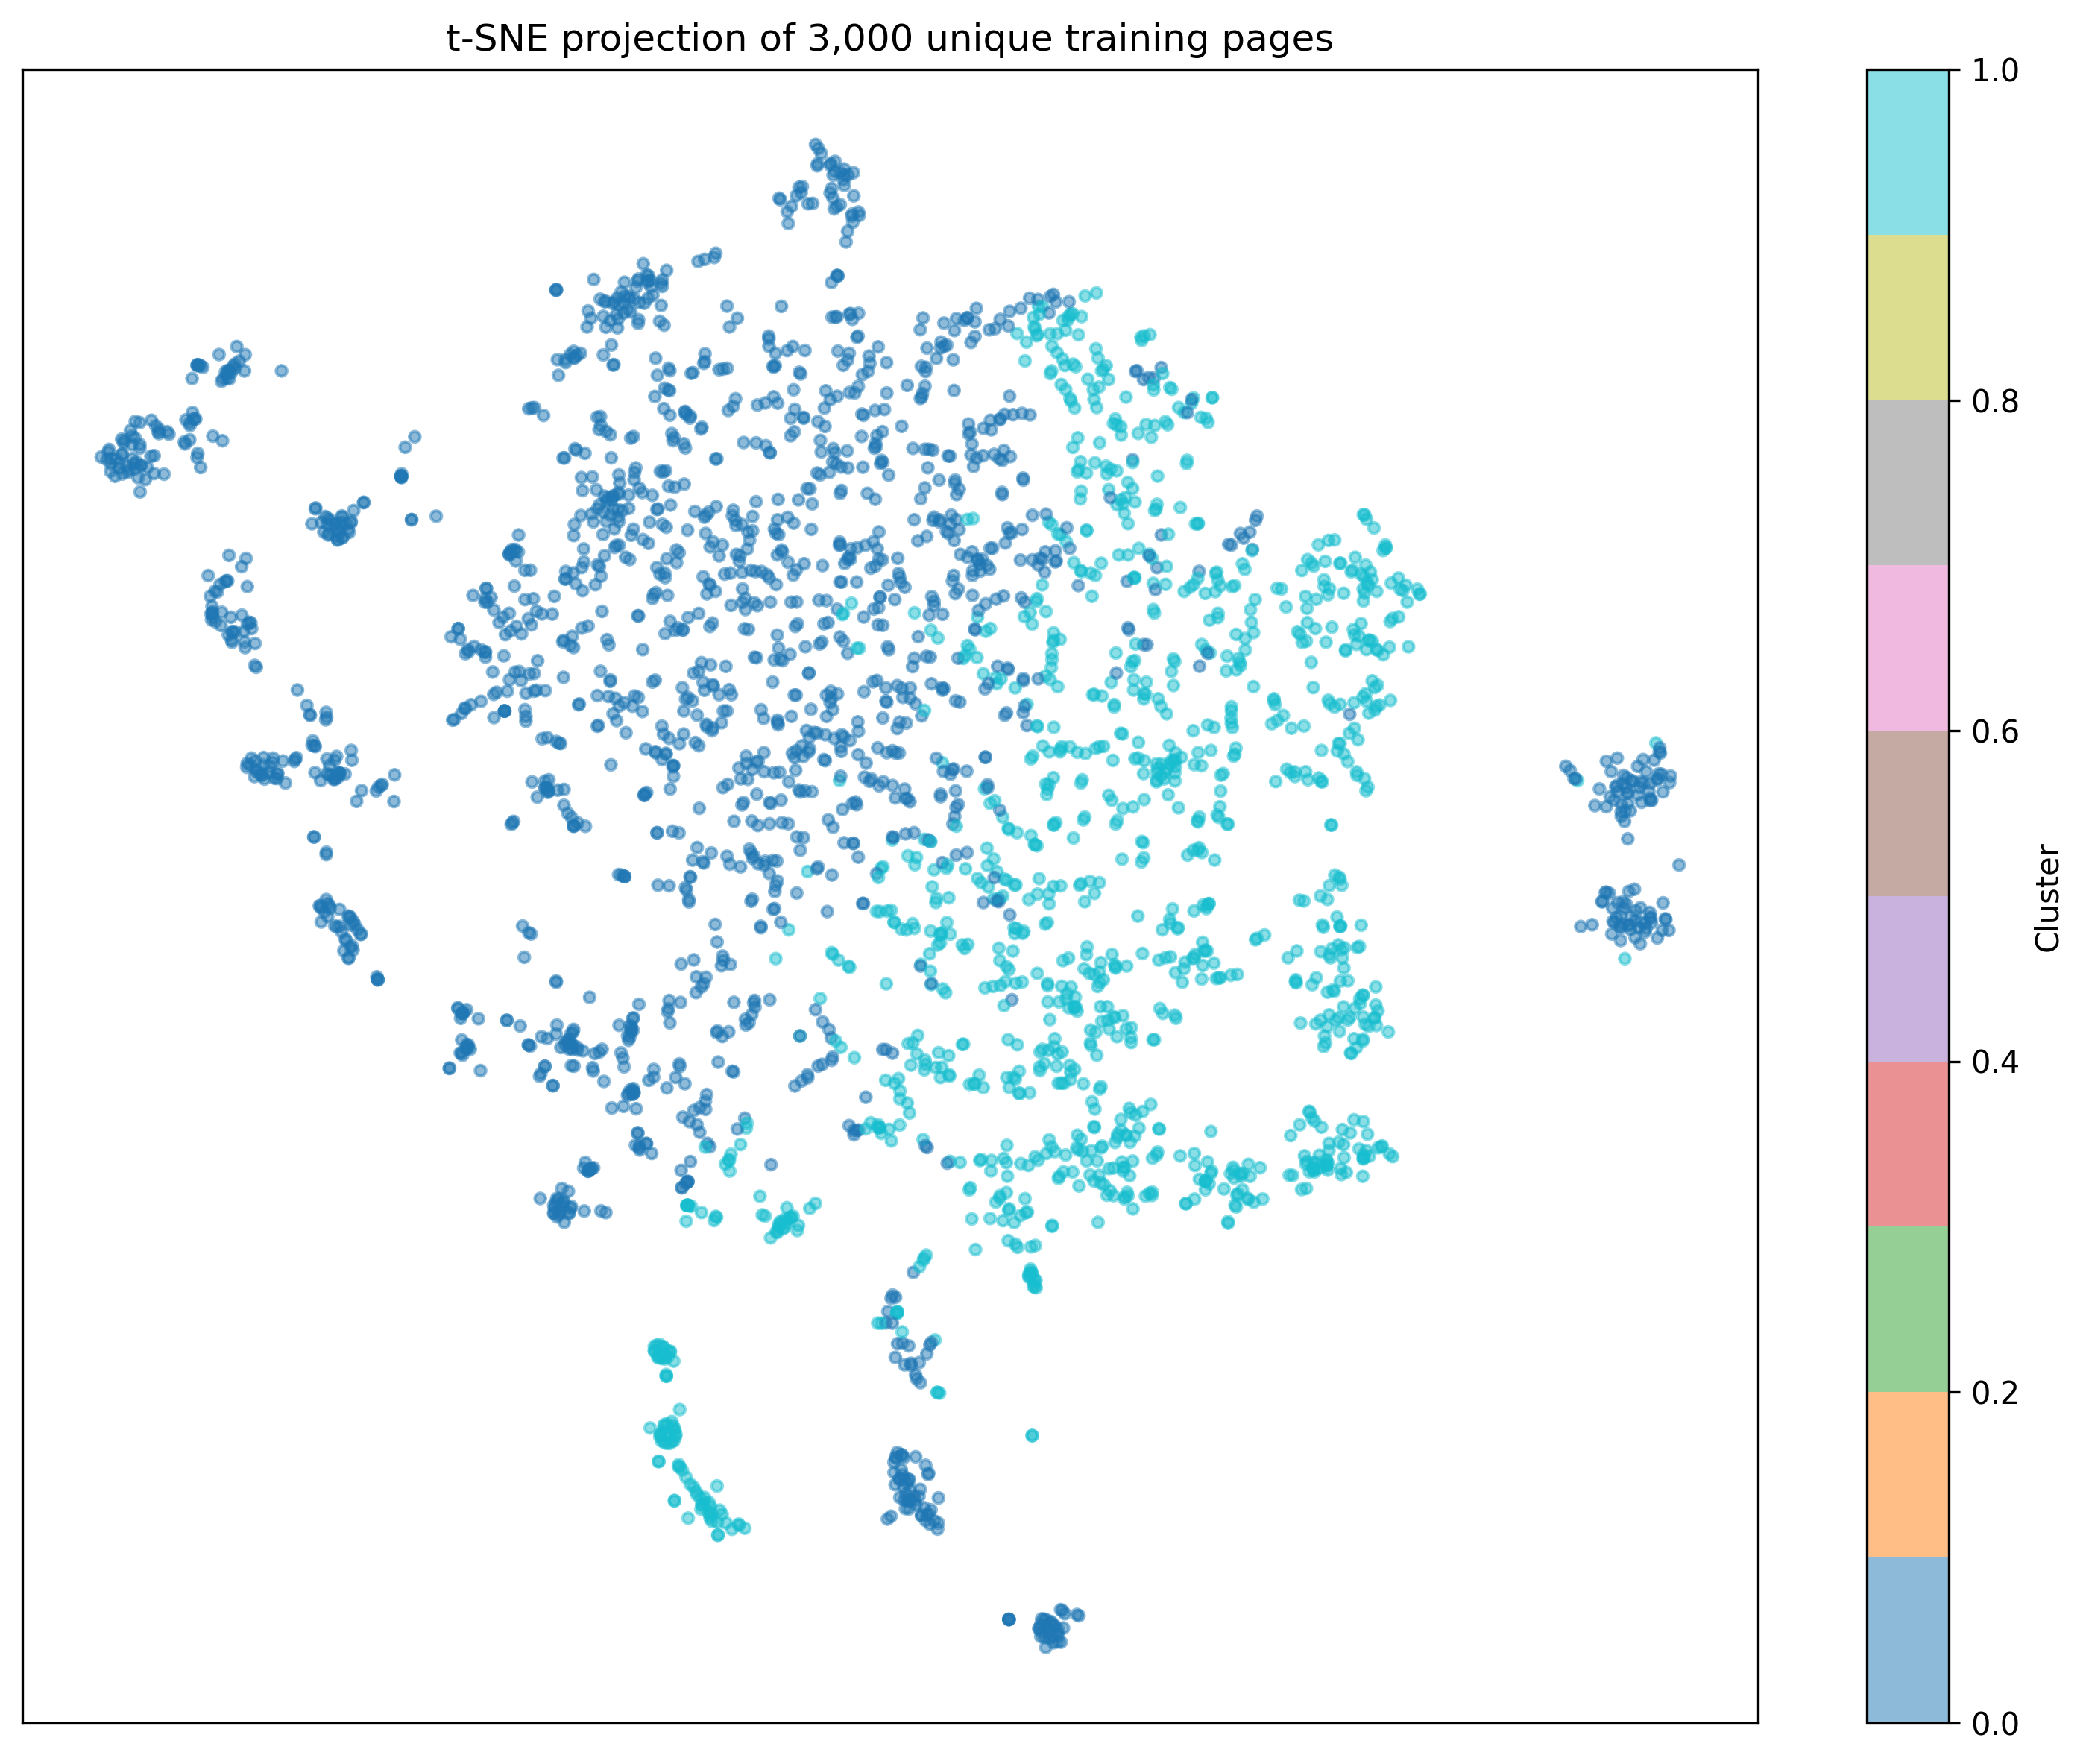
\includegraphics[width=0.68\textwidth]{figures/tsne_clusters.png}
    \caption{Final exploratory t-SNE projection of a fixed, seeded sample of
    3{,}000 unique coordinate-bearing training pages using the same standardized
    features. It is descriptive only and was not used to select $k$.}
    \label{fig:pr-clusters-manifold}
\end{figure}

\begin{figure}[H]
    \centering
    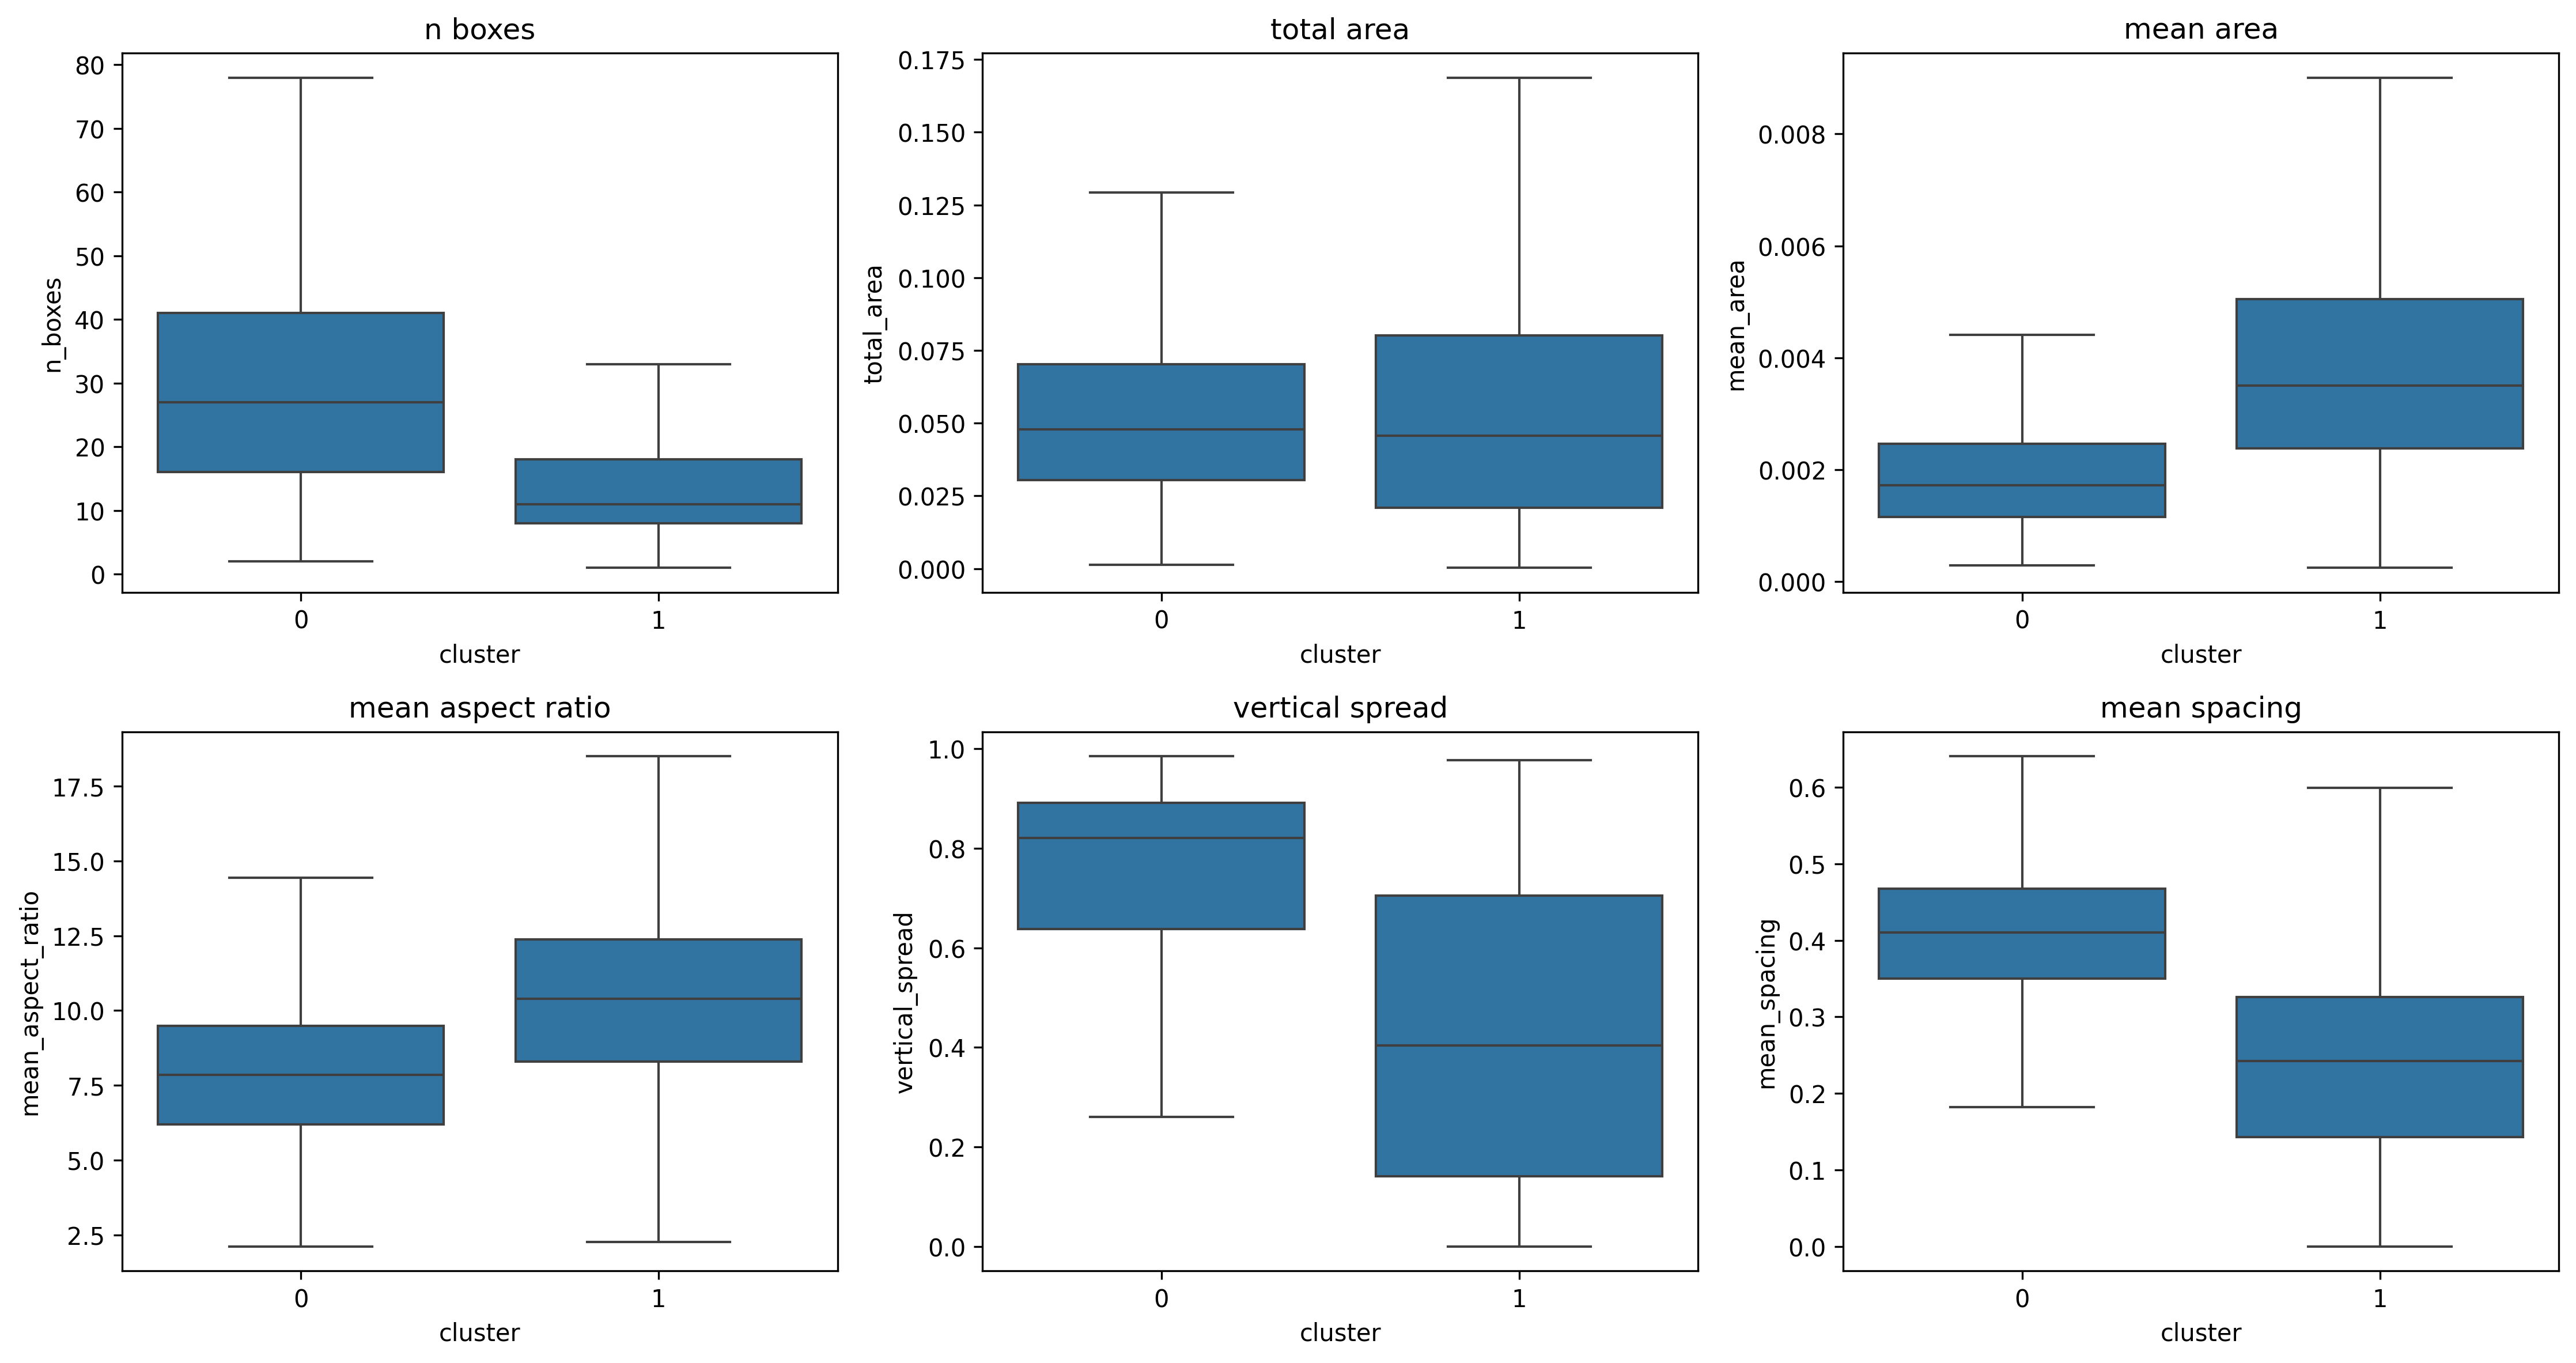
\includegraphics[width=0.84\textwidth]{figures/feature_distributions.png}
    \caption{Final selected feature distributions for the two unique-page
    annotation-geometry clusters.}
    \label{fig:pr-cluster-features}
\end{figure}

The frozen scaler and K-means model assign all 1{,}051 unique test pages as
follows: 588 to Cluster~0, 396 to Cluster~1, and 67 as geometry unavailable.
Within the 581-page prepared evaluation subset, the counts are 319, 213, and
49, respectively.

\subsection{Stage 3: Generative Baseline (Mistral-7B QLoRA)}

Mistral-7B-Instruct-v0.2 fine-tuned with 4-bit QLoRA (NF4) on LMDX-formatted document prompts. The exact prompt template is shown below. It reproduces the LMDX \emph{format and output contract} used by the KVP10k baseline (document $+$ per-word coordinates $\to$ Python list-of-lists); it is not guaranteed to be token-identical to the paper's unpublished prompt, and word text/coordinates come from PyMuPDF rather than Tesseract OCR.

\begin{quote}\small
\begin{verbatim}
<Document>
{lmdx_text}
</Document>
<Task>
From the document, extract the text keys and values.
Please provide the response in the form of a Python list of lists.
Each inner list should contain exactly two strings: the first string
is the key and the second string is the value.
Each key and value should be followed by its bounding box in the
format: left|top|right|bottom.
</Task>
### Response:
\end{verbatim}
\end{quote}

\begin{center}
\small
\begin{tabular}{lccccc}
\toprule
\textbf{System} & \textbf{Text P} & \textbf{Text R} & \textbf{Text F1} & \textbf{Location F1} & \textbf{Combined F1} \\
\midrule
KVP10k paper baseline & --- & --- & 0.659 & 0.650 & 0.611 \\
\textbf{Mistral-7B (ours)} & \textbf{0.488} & \textbf{0.774} & \textbf{0.598} & \textbf{0.547} & \textbf{0.521} \\
\bottomrule
\end{tabular}
\end{center}

\noindent\textbf{Official evaluation.} These are Regular macro pair metrics
from the official evaluator (NED $<0.2$; location matching IoU $\geq0.3$) on
our 581-page prepared test subset; 483 pages contain scorable Regular ground
truth. Exact Mistral text precision/recall/F1 are
0.48761/0.77418/0.59835; location F1 is 0.54711 and combined F1 is 0.52057.
For the broader All category, text/location/combined F1 are
0.51312/0.47804/0.45508.

The comparison is approximate: this implementation uses fewer prepared pages,
PyMuPDF text rather than the paper OCR pipeline, and a reconstructed prompt.
The official results therefore do not support the earlier claim that our
baseline matches or exceeds the paper. It is a re-implementation and trails the
published Regular F1 in all three modes. The validation-selected V4 checkpoint
also remains below the published Regular text F1 (0.363 versus 0.659).

\subsubsection*{Error Analysis by Cluster}

\begin{center}
\begin{tabular}{lrrrr}
\toprule
\textbf{Stratum} & \textbf{Assigned} & \textbf{Scored} & \textbf{Text F1} & \textbf{Combined F1} \\
\midrule
Cluster 0 & 319 & 304 & 0.651 & 0.569 \\
Cluster 1 & 213 & 179 & 0.498 & 0.429 \\
Geometry unavailable & 49 & 0 & --- & --- \\
\bottomrule
\end{tabular}
\end{center}

These official regular-pair macro scores were recomputed from saved predictions
and ground truth; no model was retrained. The geometry clusters do not support
claims about semantic document types. A separate pooled audit finds
unsupported-prediction rates of 37.1\% and 53.0\% for Clusters 0 and 1. In
this entity-level audit, an unsupported prediction is a predicted key or value
entity that has no ground-truth match under the audit's text-and-location
thresholds. The denominator is all predicted entities in the cluster.

\subsection{Stage 4: Discriminative Model --- Complete}

\subsubsection*{Architecture}

Stage~4 adapts a pretrained LayoutLMv3-base encoder with two task heads:
\begin{enumerate}[nosep]
  \item \textbf{Entity classifier:} A two-layer MLP classifies each token as
  \texttt{KEY}, \texttt{VALUE}, or \texttt{O}.
  \item \textbf{Relation linker:} A span-level projected scaled-dot-product
  linker combines semantic representations with spatial features to score
  key--value pairs.
\end{enumerate}
The active V4 and V5 component is not a full bilinear biaffine matrix. Both runs
use text and bounding boxes with the same constant blank visual input, so they
do not evaluate document-specific image content.

\subsubsection*{Experimental and diagnostic progression}

The Stage~4 experiments show the following progression:
\begin{itemize}[nosep]
  \item \textbf{V1 token linking:} An illustrative page produces approximately
  10{,}000 candidate token pairs and a negative-to-positive ratio near
  $500{:}1$. The preserved run has legacy pooled link F1 $=0.0082$.
  \item \textbf{V2 span linking:} Grouping tokens into spans reduces the same
  illustrative case to 225 candidates. With 15 positives, the ratio is
  approximately $14{:}1$. The preserved V2+TF diagnostic has legacy pooled
  link F1 $=0.0173$.
  \item \textbf{V4 pipeline correction:} The data and supervision audit found
  noisy span alignment, an over-strict bounding-box filter, and cross-product
  link labels. V4 corrects these faults together. Their separate effects were
  not isolated.
  \item \textbf{V5 final training:} V5 keeps the corrected V4 model and data
  pipeline but corrects optimizer-step scheduling, full-state resumption,
  class-aware entity metrics, early stopping, and checkpoint selection.
\end{itemize}

V1 and V2 are historical pooled diagnostics and are not directly comparable
with the official page-macro results below. Stage~4a has no reportable score
because no reliable checkpoint and class-aware result survive.

\paragraph{Official Regular pair results.}
The principal comparison uses V4 checkpoint~10, selected after all surviving V4
checkpoints were rescored on the fixed validation split. V5 checkpoint selection
uses validation Regular text+location macro F1. Table~\ref{tab:pr-final-regular}
reports the final test results on the same 581 prepared pages.

\begin{table}[H]
  \centering
  \caption{Final Regular macro pair F1 comparison.}
  \label{tab:pr-final-regular}
  \begin{tabular}{lccc}
    \toprule
    \textbf{System} & \textbf{Text} & \textbf{Location} & \textbf{Text+location} \\
    \midrule
    KVP10k paper baseline & 0.659 & 0.650 & 0.611 \\
    Mistral-7B re-implementation & 0.598 & 0.547 & 0.521 \\
    V4 validation-reselected checkpoint & 0.363 & 0.438 & 0.325 \\
    \textbf{V5 final checkpoint} & \textbf{0.392} & \textbf{0.446} & \textbf{0.345} \\
    \bottomrule
  \end{tabular}
\end{table}

\noindent\emph{Note:} Internal Mistral, V4, and V5 results use the same 581
pages. The published result is provided for context.

V5 improves the comparable V4 text+location result by 0.020, but the
reconstructed Mistral baseline remains stronger. Several training and selection
procedures change together, so the comparison does not identify the effect of
one correction.

\paragraph{Completed V5 run.}
V5 uses batch size 1, gradient accumulation 8, learning rate
$2\times10^{-5}$, linker-loss weight 5.0, a maximum of 30 epochs, and
early-stopping patience 10. It is warm-started from Canary~B, not from V4, and
loads 226 compatible entries: 212 encoder, 2 entity-classifier, and 12 linker
entries. The scheduler uses 607 optimizer updates per epoch and 500 warm-up
optimizer steps. Each checkpoint stores the full state required for resumption.

Epoch~10 has the best validation Regular text+location F1 ($0.342$) at optimizer
step 6{,}070. Training completes 20 epochs and 12{,}140 optimizer updates before
early stopping. The first job reaches its 24-hour limit after epoch~15; the
second job restores the complete state and finishes epochs 16--20. Total
allocated GPU time is approximately 31 hours and 19 minutes.

The corrected class-aware entity micro and macro F1 values are 0.792 and 0.772.
KEY F1 is 0.720 and VALUE F1 is 0.824. These entity results are substantially
higher than complete-pair F1, which identifies relation linking as the main
remaining internal bottleneck.

\paragraph{Post-processing recovery.}
The direct V5 decoder emits Regular linked pairs. The unchanged recovery method
adds unmatched predicted value spans as unkeyed outputs and unmatched predicted
key spans as unvalued outputs. It does not change Regular predictions or
Regular F1. Table~\ref{tab:pr-v5-recovery} separates direct and recovered
results.

\begin{table}[H]
  \centering
  \caption{V5 direct and recovered test macro F1.}
  \label{tab:pr-v5-recovery}
  \begin{tabular}{llccc}
    \toprule
    \textbf{Output} & \textbf{Category} & \textbf{Text} & \textbf{Location} & \textbf{Text+location} \\
    \midrule
    Direct & Regular & 0.392 & 0.446 & 0.345 \\
    Direct & All & 0.258 & 0.304 & 0.229 \\
    \midrule
    Recovered & Regular & 0.392 & 0.446 & 0.345 \\
    Recovered & Unkeyed & 0.175 & 0.316 & 0.162 \\
    Recovered & Unvalued & 0.298 & 0.336 & 0.276 \\
    Recovered & All & 0.292 & 0.376 & 0.261 \\
    \bottomrule
  \end{tabular}
\end{table}

Recovery raises All text+location F1 from 0.229 to 0.261 by adding
special-category coverage. The special-category scores remain below the Regular
score, so recovery is a coverage extension rather than a replacement for direct
relation prediction.

\paragraph{Cluster and qualitative findings.}
V5 Regular text+location F1 is 0.305 in Cluster~0 and 0.410 in Cluster~1.
Mistral has the opposite ordering, with 0.569 and 0.429. These results show an
association with annotation geometry, not semantic document types. Selected
qualitative cases show correct local links, plausible links to neighbouring
values, missed short values, KEY--VALUE confusion, and false entity labels on
ordinary prose. The cases are illustrative and do not establish frequencies.

% ============================================================
\section{Technical Challenges Encountered}
% ============================================================

\begin{enumerate}[leftmargin=1.5em]

\item \textbf{HPC Offline Compute Nodes.}
  FAU HPC compute nodes have no internet access. All models had to be pre-downloaded and cached; all \texttt{from\_pretrained()} calls required \texttt{local\_files\_only=True}.

\item \textbf{CUDA / PyTorch / Quantization Compatibility.}
  Resolving version conflicts between PyTorch, Transformers, and bitsandbytes for 4-bit QLoRA on CUDA~13.0.

\item \textbf{Data Preparation Pipeline.}
  Broken/inaccessible source PDFs ($\sim$45\% of pages), conflicting duplicate annotations, and reproducing IBM's workflow with PyMuPDF rather than their internal OCR tooling.

\item \textbf{Stage 4 Training Stability.}
  The original bilinear scorer and a bfloat16 attempt produced non-finite
  losses. The active runs use projected scaled-dot-product scoring, a valid-label
  mask before binary cross-entropy, teacher forcing, and fp32 precision.

\item \textbf{Three Compounding Data Pipeline Bugs.}
  The diagnostic work (Experiments D1--D3) required significant engineering to isolate: the bugs interacted in a way that made each individually hard to attribute. Fixing all three at once in V4 was the turning point.

\end{enumerate}

% ============================================================
\section{Literature Review Findings}
% ============================================================

\begin{itemize}[leftmargin=1.5em]
  \item \textbf{SPADE} (Hwang et al., ACL Findings 2021): spatial dependency parsing, directly inspired the spatial MLP in the Stage~4 linker.
  \item \textbf{BROS} (Hong et al., AAAI 2022): BERT-based with 2D relative position encoding and a token prediction linking head.
  \item \textbf{LMDX} (Perot et al., 2023): generative LLM approach using LMDX-formatted prompts. The approach evaluated in the KVP10k paper; published Regular text/location/combined F1 = 0.659/0.650/0.611 provides the primary comparison.
  \item \textbf{LayoutLMv3} (Huang et al., ACM MM 2022): joint text, layout,
  and image pre-training. This thesis adapts the pretrained encoder with a token
  classifier and a projected scaled-dot-product relation linker with spatial features.
\end{itemize}

% ============================================================
\section{Recent Work, Remaining Tasks, and Questions for the Supervisor}
% ============================================================

Since the previous progress report, the experimental work and principal thesis
reporting have been completed.

\subsection*{Work completed since the previous report}
\begin{enumerate}[leftmargin=1.5em]
\item \textbf{Evaluation audit and V4 reselection.}
  The released evaluator was integrated with the correct page-macro protocol,
  class-aware entity scoring was corrected, and V4 checkpoint~10 was selected
  on the fixed validation split for the principal V4 comparison.
\item \textbf{Final V5 training.}
  The corrected trainer completed 20 epochs across a full-state resume, selected
  epoch~10 by validation Regular text+location F1, and produced the final
  official test results.
\item \textbf{Final analyses.}
  Direct and recovered outputs were evaluated separately. V5 cluster results,
  corrected entity metrics, qualitative examples, run provenance, and
  checkpoint hashes were recorded.
\item \textbf{Thesis update.}
  The research questions and contributions were tightened, V5 was made the
  principal LayoutLMv3 experiment, the experimental progression was clarified,
  and the final Results, Discussion, and Conclusion chapters were updated.
\end{enumerate}

\subsection*{Remaining submission tasks}
\begin{enumerate}[leftmargin=1.5em]
\item \textbf{Overleaf compilation and bibliography.}
  Run the complete LaTeX and Biber sequence, then check citations,
  cross-references, tables, figures, and the final page layout.
\item \textbf{Final proofreading.}
  Check terminology, metric names, numerical consistency, grammar, and FAU
  formatting requirements.
\item \textbf{Supervisor review and submission.}
  Incorporate final supervisor comments and prepare the submission package for
  3 September 2026.
\end{enumerate}

\noindent\textbf{Questions for the supervisor:}
\medskip

\noindent\textbf{Scientific framing:}
\begin{enumerate}[leftmargin=1.5em]
\item Is the present text-and-layout scope acceptable without a new experiment
  using document-specific image content? The current diagnostics identify
  relation linking, rather than entity detection, as the main internal
  bottleneck.
\item Is it acceptable to retain robustness, OCR, image-rendering, and
  additional retraining experiments as future work within the remaining
  submission period?
\item Is it appropriate to present V5 as the final principal experiment and
  V1--V4 as development and diagnostic stages?
\item Is the answer to RQ3 sufficiently cautious, given that the independent
  effect of span-level linking was not isolated?
\item Are the cluster analysis and selected qualitative examples sufficient
  for the error analysis?
\end{enumerate}

\noindent\textbf{Submission procedure:}
\begin{enumerate}[leftmargin=1.5em]
\item Is code submission required with the thesis?
\item What repository access must be provided to the examiners or chair?
\item Which date must appear in the declaration?
\item What is the required final submission procedure?
\end{enumerate}

% ============================================================
\section{Timeline}
% ============================================================

\begin{center}
\begin{tabular}{llc}
\toprule
\textbf{Task} & \textbf{Status} & \textbf{Target} \\
\midrule
Stages 0--2 (data and layout analysis)       & \textcolor{completed}{\textbf{Complete}} & --- \\
Stage 3 (generative baseline)                & \textcolor{completed}{\textbf{Complete}} & --- \\
Literature review                            & \textcolor{completed}{\textbf{Complete}} & --- \\
Stage 4 implementation and V1--V5 evaluation & \textcolor{completed}{\textbf{Complete}} & --- \\
Cluster, recovery, and error analyses        & \textcolor{completed}{\textbf{Complete}} & --- \\
Principal thesis chapters                    & \textcolor{completed}{\textbf{Complete}} & --- \\
German abstract                              & \textcolor{completed}{\textbf{Complete}} & --- \\
Overleaf compilation and bibliography        & \textcolor{inprogress}{\textbf{In preparation}} & August 2026 \\
Robustness, OCR, and real-image experiments  & Descoped; future work & --- \\
Final submission                             & In preparation & 3 September 2026 \\
\bottomrule
\end{tabular}
\end{center}

% ============================================================
\section{Final Thesis Structure}
\label{sec:structure}
% ============================================================

\begin{enumerate}[nosep]
  \item \textbf{Introduction} --- Motivation, research questions, contributions
  \item \textbf{Literature Review} --- Document understanding, LayoutLM family, generative approaches (LMDX), entity linking (SPADE, BROS)
  \item \textbf{Dataset Analysis} --- KVP10k dataset, data preparation pipeline, layout clustering (before Methodology so readers understand the data first)
  \item \textbf{Methodology} --- LayoutLMv3 encoder, entity classifier, projected scaled-dot-product relation linker, training procedure, inference, and post-processing
  \item \textbf{Implementation} --- System architecture, HPC setup, training procedures
  \item \textbf{Experiments \& Results} --- Generative baseline, V1 and V2 diagnostics, corrected V4 development result, final V5 result, recovery analysis, cluster results, and qualitative errors
  \item \textbf{Discussion} --- Interpretation, generative vs.\ discriminative trade-offs, limitations
  \item \textbf{Conclusion} --- Summary of contributions, future work
\end{enumerate}

\end{document}
